\subsection*{Method}

We next moved on to develop a continuous surface erosion model. Physically this model represents a surface being worn down, such as a bar of soap in water or ice melting. 

There are a wide range of different erosion processes, and most of them are very complex. To simplify our models, all of our processes erode (move) each point along the surface in a direction normal to the surface at the point. This rarely happens in real life, because of non-homogeneous materials, nonlinear behavior, etc., but it is a reasonable assumption to make for a simplified model.

Rather than modeling erosion as a discrete process, as was done in the previous section, we can model it with the following differential equation

\begin{equation}
\label{eq:erosion-diff-eq}
\frac{d\bvec{x}}{dt} = g(\bvec{x}) \; \bhat{n}(\bvec{x})
\end{equation}

for some function $g(\bhat{x})$ to be defined shortly. $\bhat{n}(\bvec{x})$ is the unit vector normal to the surface at $\bvec{x}$.

The method used to represent the continuous surface will be explained momentarily, but first we will take a moment to explain the various erosion processes that we modeled.

The first process is a soap bar being worn down by a person holding it in their hand, which we will call our \textit{smoothing model}. In this process, the corners of the soap bar will get worn down quickest, because they are the first parts of the surface to come into contact with the person's hand. Technically the furthest protruding bumps will be worn down quickest, but to simplify the problem, we consider every point of the surface to wear down at a rate proportional to the curvature at the point. We will use a signed curvature, so that positive curvature represents an outward facing bump, and negative curvature represents an indentation in the surface. $g(\bvec{x})$ for this model is the following ($\kappa$ is the curvature)

\begin{equation}
g(\kappa(\bvec{x})) = \tan^{-1}(\beta \, (\kappa(\bvec{x}) - \alpha)) + \frac{\pi}{2}
\end{equation}

For our model we chose parameters, $\alpha = 1, \; \beta = 5$.

Our second process is an object sitting in a bath of acid, which we will call our \textit{bottom recession model}. In this process, the bottom of the object will recede quickest. $g(\bvec{x})$ for this model is the following ($x_{2, min}$ is the lowest point on the object)

\begin{align}
  f(\bvec{x})& = \frac{1}{\alpha \, (x_2 - x_{2, min}) + \beta} - \gamma\\
  g(\bvec{x})& = \begin{cases}
    f(\bvec{x}) \qquad &\text{for} \quad f(\bvec{x}) > 0\\
    0 \qquad &\text{otherwise}
  \end{cases}
\end{align}

For our model we chose parameters, $\alpha = 10, \; \beta = \gamma = 0.1$.

\subsection*{Surface Equations}

Our surface is modeled with two vectors, $x_1, x_2 \in \R^N$ for some resolution $N$. Then $\bvec{x} \coloneqq \bracket{x_1^T, x_2^T}$, with $x_1$ and $x_2$ being the two coordinates of points sampled counterclockwise along the surface.

\begin{align}
  \dot{\bvec{x}}& \coloneqq \frac{d\bvec{x}}{dt} \tag{Velocity}\\
  \ddot{\bvec{x}}& \coloneqq \frac{d^2\bvec{x}}{dt^2} \tag{Acceleration}\\
  \kappa& = \frac{\dot{\bvec{x}} \times \ddot{\bvec{x}}}{\dot{x}^3} \tag{Curvature}
\end{align}

\subsection*{Numerical Modeling}

We chose to model the surface parametrically with a Discrete Fourier series using spectral methods. Our processes tend to smooth the surfaces out over time, so spectral methods would capture this much better than a local approximation of the surface using finite differences which only act locally at points. All of our surface are in $\R^2$, so we will use the Real Fast Fourier Transform (equations in the appendix).

\begin{align}
  \dot{\bvec{x}}& = RFFT^{-1}\paren{diag(ik) \; RFFT(\bvec{x})}\\
  \ddot{\bvec{x}}& = RFFT^{-1}\paren{diag(-k^2) \; RFFT(\bvec{x})}\\
\end{align}

\begin{align}
  \bhat{n} = [-\dot{x}_2, \dot{x}_1]\\
  k& = \frac{\dot{a} \ddot{b} - \dot{b} \ddot{a}}{\paren{a^2 + b^2}^{3/2}}
\end{align}

\subsection*{Example Surface}

The example shape that we will use throughout this section is shown in Figure \ref{fig:blob-shape}.

\begin{figure}[H]
    \begin{center}
      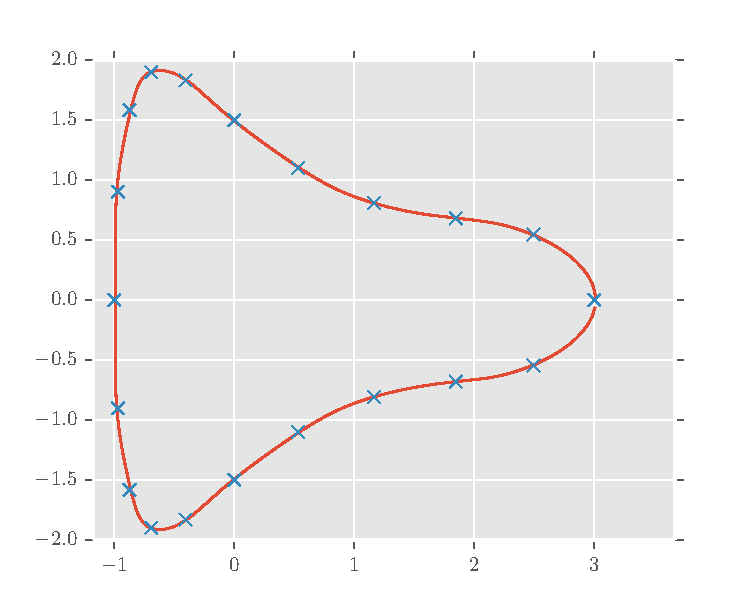
\includegraphics[keepaspectratio]{blob_shape.pdf}
    \end{center}
  \vspace{-.2in} % corrects bad spacing
  \caption{\label{fig:blob-shape} Example shape.}
\end{figure}

The equations for the shape are the following ($T_i$ is the i\textsuperscript{th} Chebyshev polynomial)

\begin{align*}
  x_1(s) = \cos(s) \paren{2 T_0(\paren{\frac{s-\pi}{\pi}}) + T_2\paren{\frac{s-\pi}{\pi}}}\\
  x_2(s) = \sin(s) \paren{2 T_0(\paren{\frac{s-\pi}{\pi}}) + T_4(\paren{\frac{s-\pi}{\pi}})}
\end{align*}

\subsection*{Point Collision Problems}

Unfortunately, the simplicity of modeling the surface with Fourier series breaks down when the surface starts to shrink. As can be seen in Figure \ref{fig:remove-lowest-blob-bad}, the process works well for a short time period, but sharp points start to form as time increases.


\begin{figure}[H]
    \begin{center}
      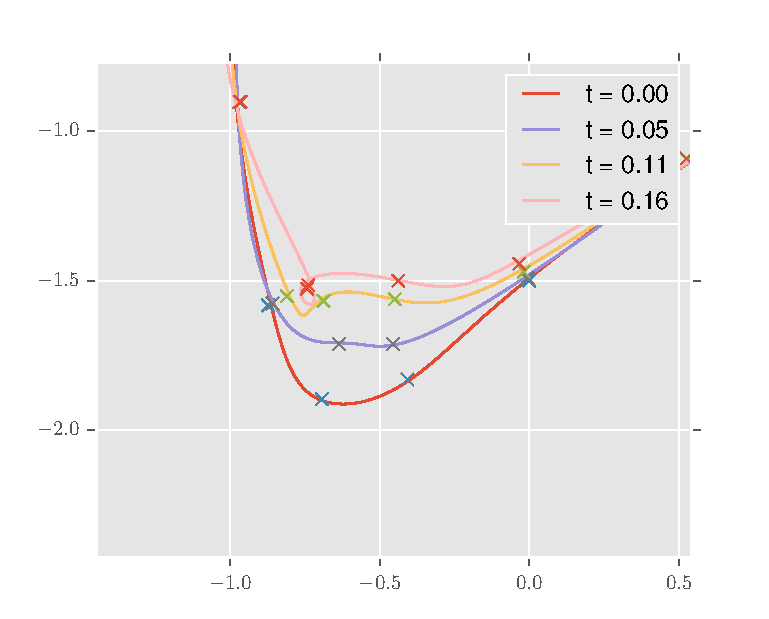
\includegraphics[keepaspectratio]{remove_lowest_blob_bad_zoom.pdf}
    \end{center}
  \vspace{-.2in} % corrects bad spacing
  \caption{\label{fig:remove-lowest-blob-bad}}
\end{figure}

To see why this occurs, we will show the same figure, but with the evaluation points shown. Looking closely, it can be seen that the sharp corners form when evaluation points get too close to each other. Our guess is that this occurs because we are using discrete time stepping, so the shape's change with time is only an approximation. This is fine when the evaluation points are far from each other, but when they get close to each other, the errors become significant and affect the direction of the surface unit normal vectors. Rather  

\begin{figure}[H]
    \begin{center}
      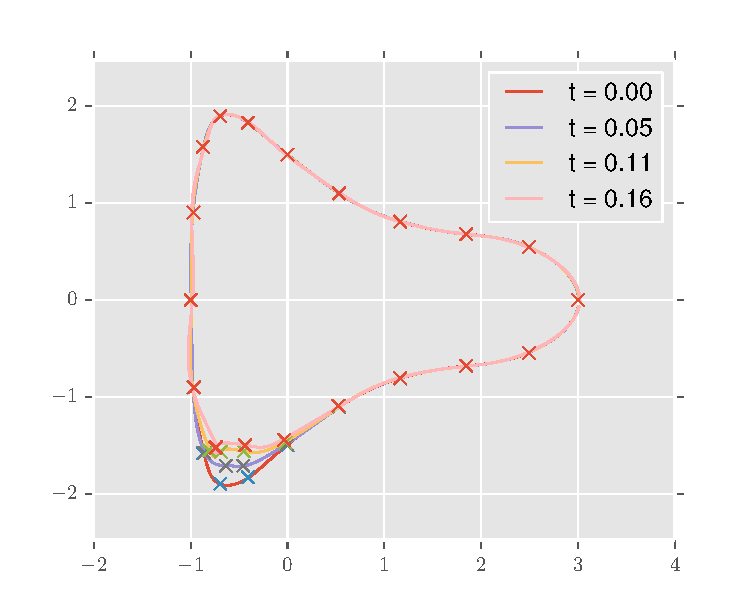
\includegraphics[keepaspectratio]{remove_lowest_blob_bad_points.pdf}
    \end{center}
  \vspace{-.2in} % corrects bad spacing
  \caption{\label{fig:remove-lowest-blog-bad-points}}
\end{figure}

\begin{figure}[H]
    \begin{center}
      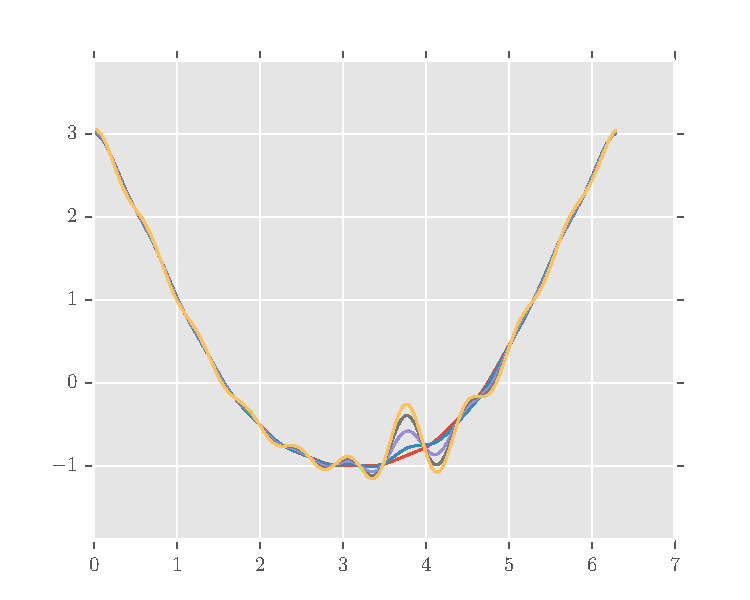
\includegraphics[keepaspectratio]{remove_lowest_blob_bad_x.pdf}
    \end{center}
  \vspace{-.2in} % corrects bad spacing
  \caption{\label{fig:remove-lowest-blob-bad-x}}
\end{figure}

\subsection*{Redistributing Points}

The most obvious way to fix this problem would be to redistribute the points evenly on the surface at every step. This wouldn't be too difficult of a task, since we can easily integrate with the FFT. 

Unfortunately, if we arbitrarily move points around, we lose spectral accuracy. Spectral methods . This method turns out to work, but I will hold off explaining it 

\subsection*{High Frequency Damping}


\subsection*{Partial High Frequency Damping}

In the \textit{erode lowest model}, 

\subsection*{Continuous Redistribution}

To redistribute points, we need to find some smooth function $f(s)$ that will map our evenly distributed $theta$. This can be achieved by 

\begin{align}
  \frac{d\bvec{x}}{dt}& = g(x) \; \bhat{n} + f(\bvec{a}_t)\\
  \bvec{a}_t& = \frac{\ddot{\bvec{x}} \cdot \dot{\bvec{x}}}{\norm{\dot{\bvec{x}}}} \; \frac{\dot{\bvec{x}}}{\norm{\dot{\bvec{x}}}}
\end{align}

$\bvec{a}_t$ is the component of $\ddot{\bvec{x}}$ tangent to the surface. $\dot{\bvec{x}}$ is inversely proportional to the density of points on the surface. We want to shift points away from denser areas, which means moving in the direction of larger $\dot{\bvec{x}}$.

As can be seen in Figure \ref{fig:remove-points-blob-good}, this dramatically improves our algorithm.

\begin{figure}[H]
    \begin{center}
      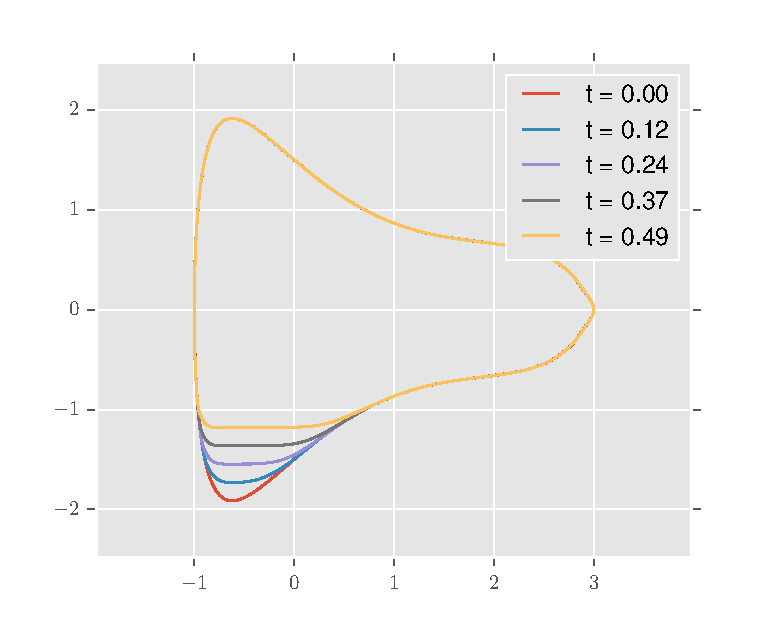
\includegraphics[keepaspectratio]{remove_points_blob_good.pdf}
    \end{center}
  \vspace{-.2in} % corrects bad spacing
  \caption{\label{fig:remove-points-blob-good}}
\end{figure}

If we plot the evaluation points (Figure \ref{fig:remove-points-blob-good-points}, it can be seen that the points redistribute themselves over time to stay evenly spaced on the surface.

\begin{figure}[H]
    \begin{center}
      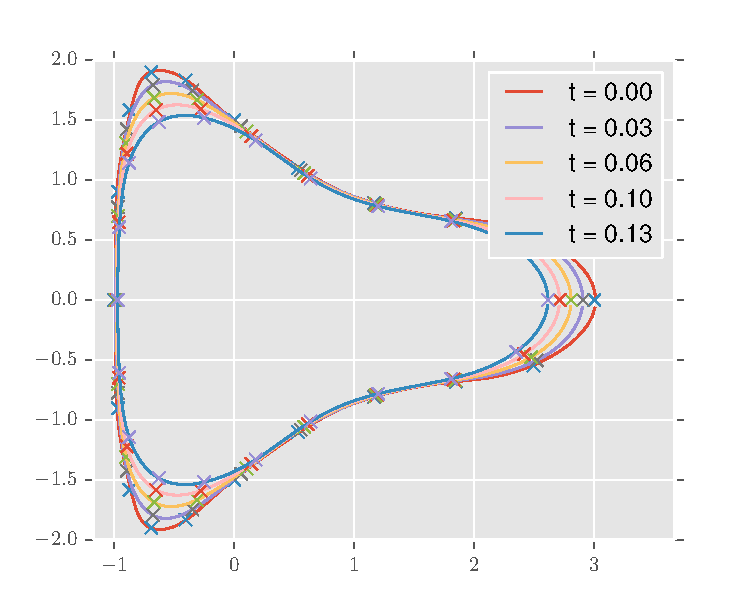
\includegraphics[keepaspectratio]{remove_points_blob_good_points.pdf}
    \end{center}
  \vspace{-.2in} % corrects bad spacing
  \caption{\label{fig:remove-points-blob-good-points}}
\end{figure}


\section*{Appendix}

\subsection*{Real Fourier Transform}

The Real Fourier transform is defined as

\begin{align*}
  \bhat{x} \coloneqq RFFT(x)_k\\
  & \coloneqq \sum_{n=0}^{N-1} e^{-2\pi i k (n/N)} x_n \qquad \text{for} \quad k = 0, \dotsc, N/2+1
\end{align*}

Note: the terms $FFT$ and Fourier transform are used interchangeably in the paper. Technically they are not synonyms, but it is common practice to use the terms interchangeably.

And the inverse transform is defined as

\begin{align*}
  x& \coloneqq RFFT^{-1}(\bhat{x})\\
  & \coloneqq \frac{1}{N} \paren{\sum_{k=0}^{N/2+1} e^{2\pi i k (n/N)} X_k + \sum_{k=N/2+2}^{N-1} e^{2\pi i k (n/N)} \bar{X}_k} \qquad \text{for} \quad n = 0, \dotsc, N-1
\end{align*}